\documentclass[11pt,a4paper]{article}

\usepackage{style2017}
\usepackage{hyperref}
\usepackage{listings}
\definecolor{codegreen}{rgb}{0,0.5,0}
\definecolor{codegray}{rgb}{0.5,0.5,0.5}
\definecolor{codepurple}{rgb}{0.58,0,0.82}
\definecolor{backcolour}{rgb}{0.95,0.95,0.92}
\lstset{
	language=python,
	frame=single,
	xleftmargin=2em,
	xrightmargin=2em,
	%backgroundcolor=\color{backcolour},   
    commentstyle=\color{codegreen},
    keywordstyle=\color{codegreen},
    numberstyle=\color{black!80!white},
    stringstyle=\color{blue},
    basicstyle=\ttfamily,
    %columns=[l]flexible,
    breakatwhitespace=false,         
    breaklines=true,                 
    captionpos=b,                    
    keepspaces=true,                 
    %numbers=none,                    
    %numbersep=1em,               
    showspaces=false,                
    showstringspaces=false,
    showtabs=false,                  
    tabsize=2,
    emph={False,True},
    emphstyle=\color{codegreen}
}

\hypersetup{
    colorlinks =false,
    linkcolor=blue,
   linkbordercolor = 1 0 0
}
\newcounter{numexo}
\setcellgapes{1pt}

\begin{document}



\begin{NSI}
{Exercice}{Chaines de caractères et listes}
\end{NSI}



%\addtocounter{numexo}{1}
%\subsection*{\Large Exercice \thenumexo }

En python, les chaines de caractères peuvent être traitées comme des listes de lettres. \medskip

Par exemple, la chaine de caractères \textsf{'python'} est aussi la liste \textsf{['p', 'y', 't', 'h', 'o', 'n']}.\medskip


Les palindromes sont des mots ou expressions qui peuvent se lire de gauche à droite ou de droite à gauche en ayant le même sens. Par exemple, le mot \textsf{kayak} est un palindrome.

\begin{enumerate}
\item On donne le code de la fonction \textsf{renverse} qui prend en paramètre une chaine de caractères et renvoie une chaine de caractères.

\begin{lstlisting}
def renverse(ch1):
	ch2 = ''
	for lettre in ch1:
		ch2 = lettre + ch2
	return ch2
\end{lstlisting}

\begin{enumerate}
\item Que renvoie l'appel de la fonction \textsf{renverse("chaine")} ?
\item Que renvoie l'appel de la fonction \textsf{renverse("elu par cette crapule")} ?
\end{enumerate}
\item La fonction \textsf{palindrome} prend en paramètre une chaine de caractères et renvoie un booléen. La fonction renvoie \textsf{True} si la chaine de caractères est un palindrome et \textsf{False} sinon.
\begin{enumerate}
\item Écrire en Python la fonction \textsf{palindrome}. On utilisera la fonction \textsf{renverse}.
\item Vérifier votre fonction avec les chaines de caractères \textsf{'non'}, \textsf{'kayak'} et \textsf{'infini'}.
\item Que renvoie la fonction avec la chaine de caractères \textsf{'elu par cette crapule'}. Expliquer pourquoi.
\end{enumerate}
\item Une première solution consiste à supprimer les espaces de la chaine de caractères dans la fonction \textsf{palindrome}.
\end{enumerate}


%\addtocounter{numexo}{1}
%\subsection*{\Large Exercice \thenumexo }
%\begin{enumerate}
%\item Créer deux tableaux \textbf{jours} et \textbf{mois} regroupant toutes les valeurs possibles.
%\item Créer la fonction \textbf{affiche\_janvier} affichant tout le mois de janvier commençant par un lundi 1 janvier.
%\item Modifier la fonction \textbf{affiche\_janvier} prenant en paramètre le premier jour du mois (lundi, mardi, mercredi,...) et affichant le mois en conséquence.
%\item Créer la fonction \textbf{affiche\_mois} prenant comme paramètre un mois et le premier jour du mois et affichant le mois. On prendra en compte le nombre de jours dans le mois.
%\item Écrire une fonction \textbf{est\_bissextile} prenant en paramètre l'année et retourne \textbf{True} si elle est bissextile ou \textbf{False} dans le cas contraire. On rappelle qu'une année est bissextile si elle est un multiple de 4 mais pas un multiple de 100, ou si elle est un multiple de 400.
%\item Modifier la fonction \textbf{affiche\_mois} en ajoutant comme paramètre l'année et affichant le mois de février avec 28 ou 29 jours.
%\item Modifier la fonction \textbf{affiche\_mois} pour qu'elle retourne un tableau des dates demandées.
%\end{enumerate}
%
%
%
%\addtocounter{numexo}{1}
%\subsection*{\Large Exercice \thenumexo }
%\begin{enumerate}
%\item Créer une fonction \textbf{nouvelleGrille} qui crée un tableau de tableaux de dimension $10 \times 10$, c'est à dire de $10$ lignes et $10$ colonnes initialisée avec des zéros.\\
%Créer la variable \textbf{maGrille} qui est une grille $10 \times 10$ de zéros.
%\item Créer une fonction \textbf{alimente} qui remplit la grille avec des nombres entiers aléatoirement choisis entre 0 et 200. Alimenter la variable ma\_grille.
%\item Créer une fonction \textbf{tabmax} qui renvoie la plus grande valeur d'un tableau (voir exercice 2).
%\item Créer une fonction \textbf{transpose} qui prend en paramètre une grille et renvoie une grille dont les lignes sont les colonnes de la grille saisie en paramètre.
%\item Créer une fonction \textbf{maxiligne} qui renvoie un tableau contenant la valeur maximale de chaque ligne de la grille. Penser à utiliser la fonction tabmax.
%\item Créer une fonction \textbf{maxicolonne} qui renvoie un tableau contenant la valeur maximale de chaque colonne de la grille. Penser à utiliser la fonction tabmax et la fonction transpose.
%\end{enumerate}
%
%\newpage
%\addtocounter{numexo}{1}
%\subsection*{\Large Exercice \thenumexo }
%Le Verger est un jeu de société coopératif créé en 1986. Ce jeu contient:
%\begin{itemize}
%\item un plan de jeu présentant 4 arbres fruitiers (prunier, pommier, poirier, cerisier) ainsi qu'un corbeau au centre.
%\item 40 fruits (10 pour chaque arbre du plan de jeu) en bois à disposer sur chacun des arbres.
%\item 4 paniers pour les joueurs (1 panier par joueur)
%\item Un puzzle corbeau de 9 pièces que l'on reconstitue lors de la partie.
%\item Un dé dont les faces représentent les 4 arbres, le panier et le corbeau.
%\end{itemize}
%
%\begin{center}
%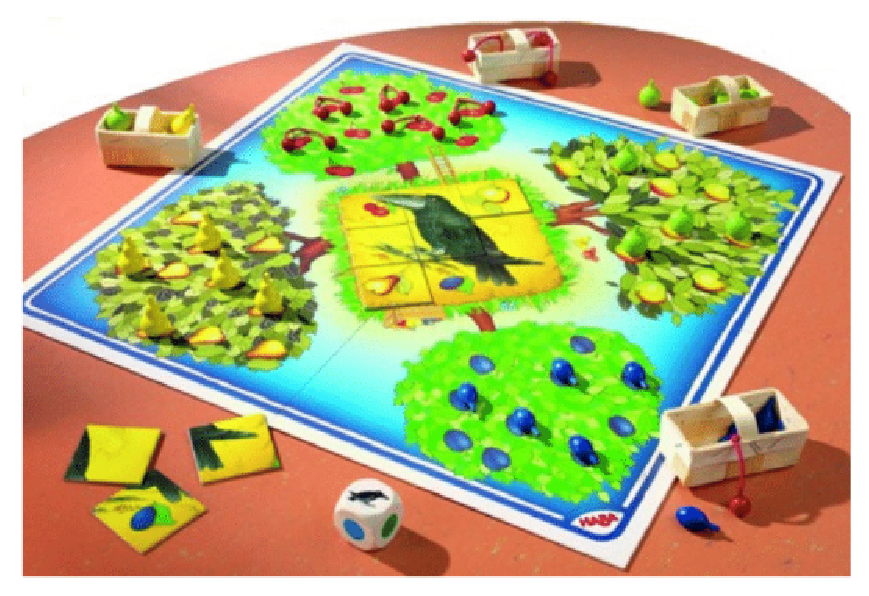
\includegraphics[scale=0.5]{img/verger.eps}
%\end{center}
%
%\subsubsection*{Règles du jeu}
%Le but du jeu est de récupérer tous les fruits avant d'avoir reconstitué le puzzle du corbeau.
%
%Un joueur lance le dé :
%\begin{itemize}
%\item Si le dé tombe sur un arbre, le joueur prend le fruit correspondant et le met dans son panier. S'il n'y a plus de fruit sur l'arbre, le joueur passe son tour.
%\item Si le dé tombe sur le panier, le joueur prend 2 fruits de son choix.
%\item Si le dé tombe sur le corbeau, il place une pièce du puzzle sur le corbeau.
%\end{itemize}
%
%\subsubsection*{Le gagnant}
%Les joueurs gagnent tous ensemble s'ils ont réussi à cueillir tous les fruits de tous les arbres.
%Les joueurs perdent ensemble si le puzzle du corbeau est reconstitué avant d'avoir cueilli tous les fruits.
%
%\subsubsection*{Programmation}
%Écrire un programme qui permet d'effectuer une partie et affiche le gagnant.
%
%
%\newpage
%\addtocounter{numexo}{1}
%\subsection*{\Large Exercice \thenumexo }
%Le jeu du loto se joue avec des grilles différentes composées de 15 numéros compris entre 1 et 90 (inclus). Au cours d'une partie, des numéros sont tirés au hasard. Le premier à avoir une grille complète est le gagnant du lot principal.
%
%On donne un exemple de grille ci-dessous:
%
%\begin{center}
%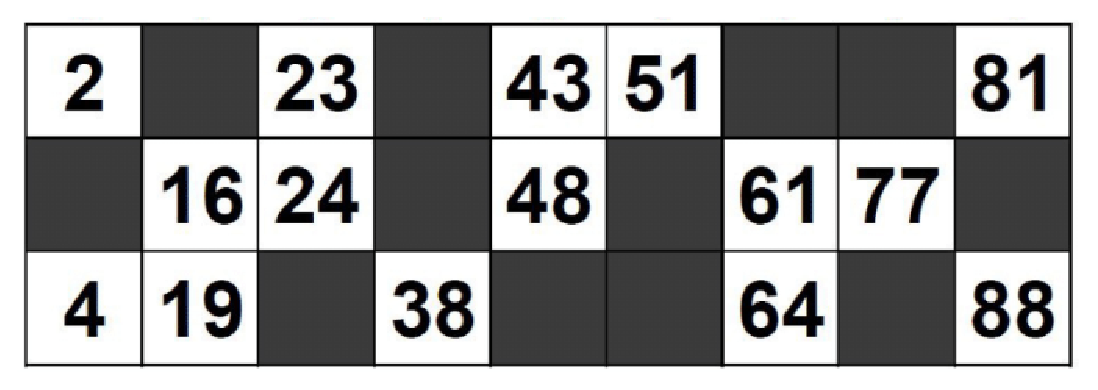
\includegraphics[scale=0.6]{img/loto.eps}
%\end{center}
%
%Écrire un programme produisant une carte de loto en respectant les contraintes suivantes :
%\begin{itemize}
%\item Une carte contient 9 colonnes et 3 lignes.
%\item Il y a sur la carte 15 numéros différents choisis parmi les nombres de 1 à 90.
%\item Chaque ligne contient 5 numéros (et donc 4 espaces vides).
%\item Il y a toujours au moins un numéro par colonne.
%\item Il peut y avoir 3 numéros dans une colonne, mais seulement dans la colonne 8.
%\item La colonne 0 contient les numéros de 1 à 9.
%\item La colonne 1 contient les numéros de 10 à 19.
%\item La colonne 2 contient les numéros de 20 à 29.
%\item ...
%\item La colonne 8 contient les numéros de 80 à 90.
%\end{itemize}


\end{document}

